\chapter{Evaluation}

Evaluating the results of bandwidth limitations is more difficult than it might seem. Both, bandwidth limitation utilities like \acs{TC} as well as testing tools like iPerf3 are often hard to configure correctly and are sometimes documented quite incomprehensibly. Therefore, it is often unclear whether errors are measurement errors or limitation errors. Furthermore, there is no such thing as standard \acs{IP}- or even \ac{UDP}-traffic. Packets can have different sizes, can be reordered or get lost. All those factors can influence and sometimes falsify the measurement. And finally it is questionable whether the traffic that is generated by the testing tools is similar enough to normal traffic generated by an \acs{AS}, such that we can conclude anything meaningful.
\\
What is known about the environment in which the \textit{scionlab\_bw\_limiter} will be running is that we deal with \acs{UDP}-traffic over \acs{IP}v4 and at some point in the future might be dealing with \acs{IP}v6 traffic as well. Therefore, we mainly focus on testing the bandwidth limitations using \acs{UDP}-traffic over \acs{IP}v4. However, note that the \textit{scionlab\_bw\_limiter} also works with \acs{IP}v6 traffic and that the test results look almost identical to the test results when using \acs{IP}v4 traffic.
\\
In this chapter we will first discuss the general test set-up, then a first test approach will be presented, which shows some unexpected anomalies. In section \ref{Examination of the Problem with Ingress Traffic}, we will examine the cause for these anomalies. From the  knowledge gained from this examination, we deduce a realistic test configuration that delivers the results that we expect and that proves the effectiveness of the \textit{scionlab\_bw\_limiter}. The final results are presented in figure \ref{Evaluation of the Bandwidth with a Datagram Size of 1500 Bytes (Size of the MTU)}.

\newpage

\section{Test Set-up}

As a test set-up it makes sense to have a test server, which doesn't have any bandwidth limitations and a test client, where the \textit{scionlab\_bw\_limiter} will enforce the desired bandwidth limits. As a test client I decided to use my development \acs{VM}, which I also use to develop and test the \textit{scionlab\_bw\_limiter}. This \acs{VM} runs Ubuntu 18.04, which is a newer version than the one running on the \aclp{AP}, but since \acs{TC} works the same way on both versions of Ubuntu, this should not matter. The test server is a Ubuntu 18.04 server that runs in a \acs{VM} as well and is hosted on the same physical machine as the test client. Therefore traffic between the test server and the test client is not real network traffic, but since the \acs{TC} configurations are effective between the Linux kernel and the network driver, where both of which are virtualized, the \acs{TC} configurations should have the exact same effect in this setting as in the real environment.

\subsection{Set-Up Using iPerf3}

I installed iPerf3 on both the test client as well as on the test server and let the test server run iPerf3 as a server. Note that the same software is used for both the server side as well as the client side. They just run in different modes. On the client I can now connect to the test server and run highly customisable tests with the server. Normally the client is the one sending data to the server, but iPerf3 can be run in a reverse mode (using the \textit{-R} option), such that we can test both ingress as well as egress traffic without having to switch between client and server mode on our machines.

\section{iPerf3}

iPerf3 is a state of the art network performance measurement tool. It is a successor of iPerf and iPerf2. However it has been completely rewritten in order to make the code base cleaner and simpler and is therefore not backward compatible with iPerf2. iPerf3 has been developed by \ac{ESnet}, which is a high-speed computer network provider for the United States Department of Energy. iPerf3 is open-source and can be found on \href{https://github.com/esnet/iperf}{github.com}\cite{mah2018iperf3}.
\\
iPerf3 can test both \ac{TCP} as well as \acs{UDP} traffic. In our case we only need to test \acs{UDP} traffic. This can be done by passing the option \textit{-u} as an argument to iPerf3. When running it we need to specify a target bandwidth (option \textit{-b}). iPerf3 then tries to achieve this bandwidth by sending traffic out at this rate. To run iPerf3 in server mode we only have to pass \textit{-s} as an argument. For running it in the client mode we have to analogously pass the \textit{-c} option followed by the server's \acs{IP}-address. Last but not least, we can optionally set the buffer length of the buffer from which is sent and to which is received by passing the option \textit{-l} followed by a size in bytes as an argument. This will determine the size of the datagrams that are being sent. As we will see in section \ref{Test Results}, this option is of quite a significance.

\section{Test Results}\label{Test Results}

The following test results occurred under the following configuration:
\\
The server's \acs{IP}-address is in our case 192.168.17.129, the \acs{IP}-connection to the server is limited to 500Kbps and the default bandwidth is 1000Kbps. The \ac{MTU} parameter in \acs{TC} is set to the \acs{MTU} of the network interface that is used to connect to the specific \acs{IP}-address. In our case this is 1500 bytes. The burst parameter, which is the size of the bucket in the \acs{TBF} algorithm is set to 5K. The ceil rate is the same as the normal rate, which is 500Kbps to the test server and 1000Kbps to any other \acs{IP}-device that uses the same interface.
\\
\\
On the test server, we start iPerf3 using no other options than the \textit{-s} option, that makes iPerf3 run in server mode (see listing \ref{Test Server Command}). On the client side, we configure a bit more. We set the client into client mode using the \textit{-c} option followed by the server's \acs{IP}-address. Furthermore, we set the \textit{-u} option, in order to generate \acs{UDP} traffic as test traffic. The target bandwidth is set to 2Mbps (option \textit{-b}) and the only parameter that we are going to change for different tests is the datagram size (option \textit{-l}). We start at a size of 1000 bytes and go up to 10000 bytes. And finally we set the \textit{-R} option in case we want to run the test in reverse mode, meaning that we test with ingress traffic. Listings \ref{Example Egress Test Command} and \ref{Example Ingress Test Command} show what these commands look like. Note that if we set the datagram size too small, we encounter an error. This happens because the packets arrive in a different order than they were sent. Therefore iPerf3 can't measure the bandwidth any more. This phenomenon is discussed on \href{https://github.com/esnet/iperf/issues/457}{github.com}\cite{mah2016iperfIssue} in the issues section of the iPerf repository.

\newpage

\begin{lstlisting}[language=sh, caption = Test Server Command, captionpos=b, numbers=left, frame=single, breaklines=true, breakatwhitespace=true, showstringspaces=false, label=Test Server Command]
iperf3 -s
\end{lstlisting}

\begin{lstlisting}[language=sh, caption = Example Egress Test Command, captionpos=b, numbers=left, frame=single, breaklines=true, breakatwhitespace=true, showstringspaces=false, label=Example Egress Test Command]
iperf3 -c 192.168.17.129 -u -b 2Mbit -l 1000
\end{lstlisting}

\begin{lstlisting}[language=sh, caption = Example Ingress Test Command, captionpos=b, numbers=left, frame=single, breaklines=true, breakatwhitespace=true, showstringspaces=false, label=Example Ingress Test Command]
iperf3 -c 192.168.17.129 -u -b 2Mbit -l 1000 -R
\end{lstlisting}

\subsection{Interpretation of the Test Results}

Figure \ref{Evaluation of the Bandwidth} shows the average bandwidth over ten samples for both ingress as well as egress traffic with respect to the datagram size. For the egress traffic the results look quite good. The average egress bandwidth lies slightly above the bandwidth limit. This is because we allow short bursts at a higher speed. Therefore, the limitations on egress traffic can be considered as effective and stable.
\\
However, for ingress traffic it is a bit a different story. That the ingress bandwidth is lower than the egress bandwidth is expected, because there is a slight overhead caused by redirecting ingress traffic from a physical interface to a virtual interface. So having a situation like we have it with a datagram size of 1000 bytes would be desirable. However, we can't ignore that by increasing the datagram size, the ingress bandwidth drops quite drastically. For getting on the bottom of this issue, let us consider figure \ref{Evaluation of the Bandwidth Drops}. This figure shows the number of samples at a bandwidth of zero depending on the size of the datagram. It is visible that the bigger the datagram, the more the ingress traffic suffers from samples with a bandwidth of zero. This phenomenon happens with egress traffic as well, but there it is much less significant. The increasing number of zero bandwidth samples shows that the decreased average bandwidth is not caused by a wrong limitation, since the samples that make it through are received at a bandwidth that is around the desired limit, but that for some samples either iPerf3 fails to do a measurement at all or something prevents the machine from receiving data for some time. To figure out whether these anomalies are the result of side effects the \textit{scionlab\_bw\_limiter} causes or are measurement errors of iPerf3 or reflect normal behaviour of traffic under the current test configuration, we need to compare these results with results we get if we enforce a bandwidth limit using a different tool.

\begin{figure}[h]
	\centering
	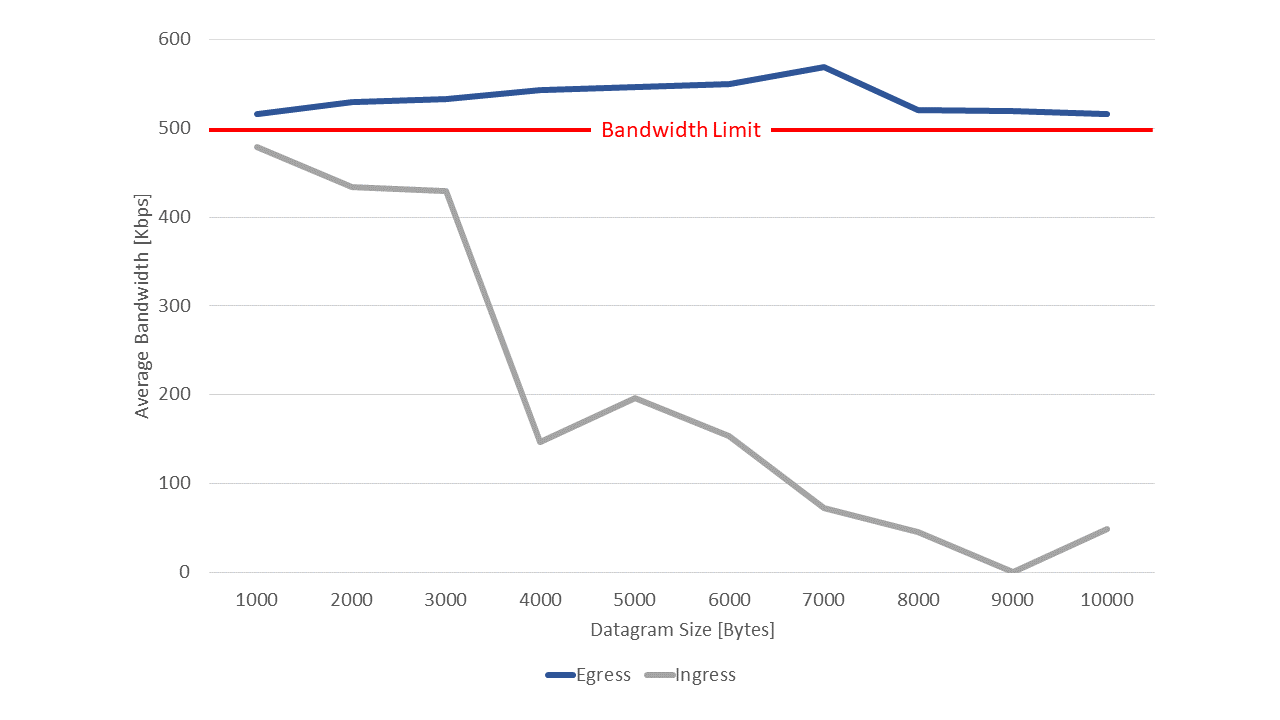
\includegraphics[width=\textwidth]{img/Evaluation-Bandwidth.png}
	\caption{Evaluation of the Bandwidth}
	\label{Evaluation of the Bandwidth}
\end{figure}

\begin{figure}[h]
	\centering
	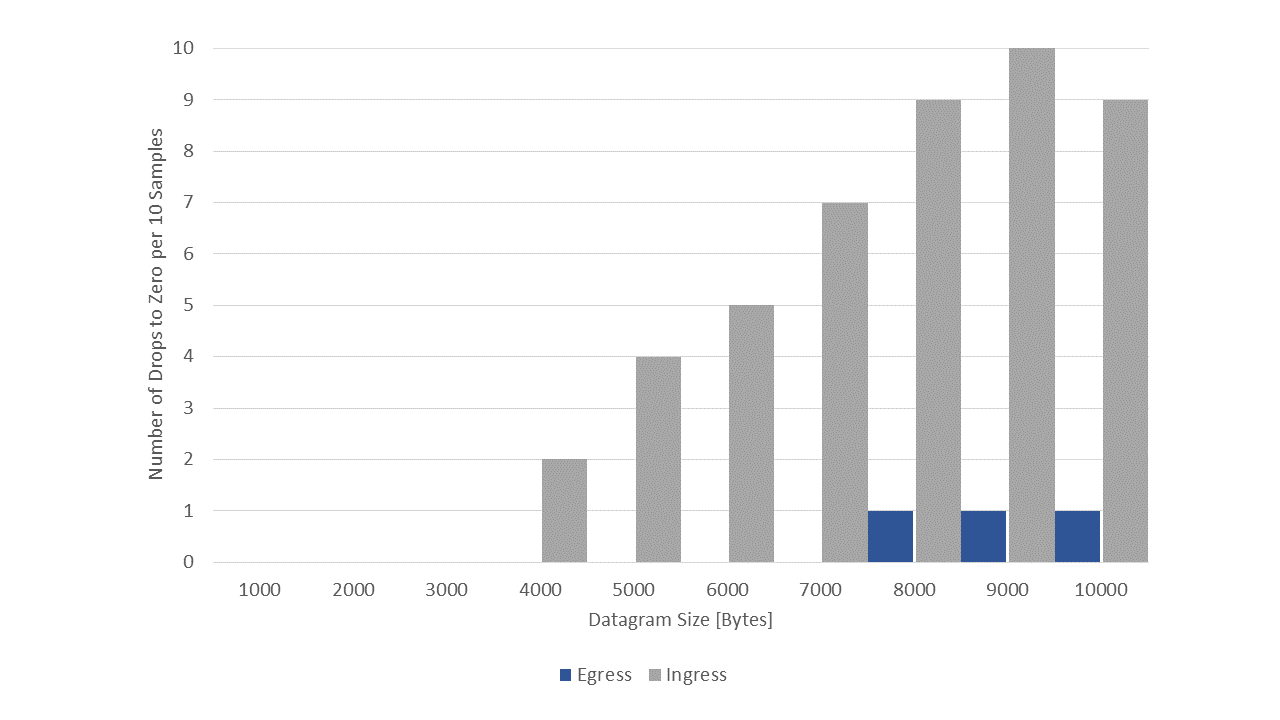
\includegraphics[width=\textwidth]{img/Evaluation-Zeros.png}
	\caption{Evaluation of Bandwidth Drops}
	\label{Evaluation of the Bandwidth Drops}
\end{figure}

\newpage
\textit{ }
\newpage

\subsection{Comparison with Wondershaper}

\textit{Wondershaper} is an open-source program that has been developed by some of the major contributors of the \textit{Linux advanced routing \& traffic control HOWTO}\cite
{hubert2002linux}. The code of \textit{wondershaper} can be found on \href{https://github.com/magnific0/wondershaper}{github.com}\cite{hubert2002wondershaper}. \textit{Wondershaper} only allows the user to enforce a general bandwidth limit and not individual bandwidth limits per \acs{IP}-address. On the other hand it allows us to set an ingress bandwidth that is different from the egress bandwidth. But since we don't require that, we just set the same bandwidth limits in both cases on the interface that is used to connect to the test server. Listing \ref{Wondershaper command} shows the command that has been used in order to enforce a bandwidth limit of 500Kbps on interface \textit{ens33}.

\begin{lstlisting}[language=sh, caption = Wondershaper command, captionpos=b, numbers=left, frame=single, breaklines=true, breakatwhitespace=true, showstringspaces=false, label=Wondershaper command]
sudo ./wondershaper -a ens33 -u 500 -d 500
\end{lstlisting}

As we can se in Figure \ref{Evaluation of the Bandwidth (Wondershaper)} and \ref{Evaluation of the Bandwidth Drops (Wondershaper)} the same phenomenon occurs if we enforce a bandwidth limit with \textit{wondershaper} and run the exact same tests as before. It is worth noticing that even though the test results for ingress traffic look similarly bad, yet quite different from the results from the \textit{scionlab\_bw\_limiter}, both \textit{wondershaper} as well as the \textit{scionlab\_bw\_limiter} use the \acs{IFB} interfaces and the \textit{ingress} \acs{QDISC} and are therefore implemented almost equivalently. The egress bandwidth limits however are implemented quite differently even though the test results look almost the same. When it comes to egress traffic, \textit{wondershaper} distinguishes between different types of service, in order to achieve a better quality of service. In our case this is not necessary, since we are not dealing with average "every day traffic", but only with \acs{SCION} traffic that is wrapped into \acs{IP} packets.  

\begin{figure}[h]
	\centering
	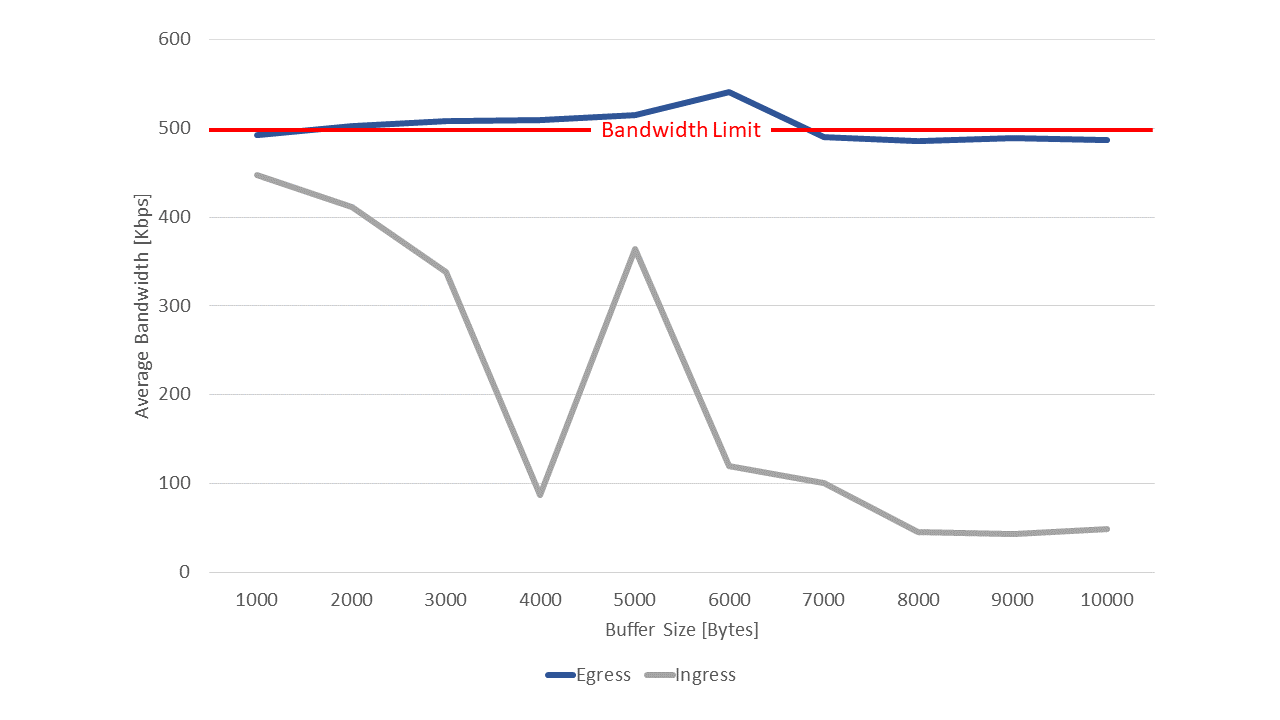
\includegraphics[width=\textwidth]{img/Evaluation-Bandwidth-Wondershaper.png}
	\caption{Evaluation of the Bandwidth (Wondershaper)}
	\label{Evaluation of the Bandwidth (Wondershaper)}
\end{figure}

\begin{figure}[h]
	\centering
	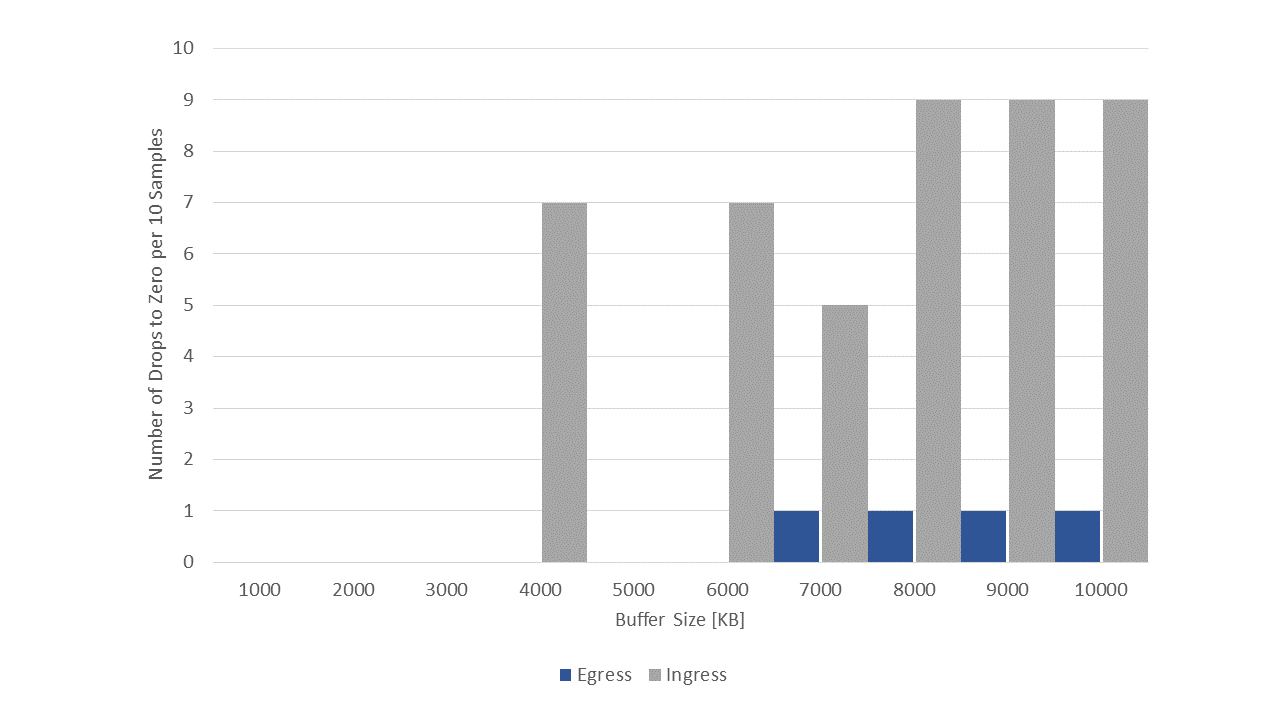
\includegraphics[width=\textwidth]{img/Evaluation-Zeros-Wondershaper.png}
	\caption{Evaluation of Bandwidth Drops (Wondershaper)}
	\label{Evaluation of the Bandwidth Drops (Wondershaper)}
\end{figure}

\newpage

\subsection{Examination of the Problem with Ingress Traffic}\label{Examination of the Problem with Ingress Traffic}

If the size of a datagram that is being sent by iPerf3 in order to determine the bandwidth is bigger than the \acs{MTU}, then fragmentation happens. The \acl{IP} itself doesn't handle the loss of packets. This is the responsibility of protocols higher above in the \acs{OSI} model. In our case, we have \acs{UDP} as a  \acs{OSI}-layer 4 protocol. In \acs{UDP}, if a fragment gets lost, then the entire packet is considered lost. Bandwidth limitations using \acs{TC} on egress traffic happen before the datagrams get fragmented and on ingress traffic, the reassembly of the fragments happens after the \acs{TC} configurations had their effect (see figure \ref{Schematic Representation of where Fragmentation occurs} for further clarification). This leads to the hypothesis that if iPerf3 sends datagrams that need to be fragmented and tries to send them at a speed that is higher than the enforced bandwidth limit, we measure a significant drop in bandwidth, because some fragments of the datagram get dropped and therefore the entire datagram gets dropped.

\begin{figure}[h]
	\centering
	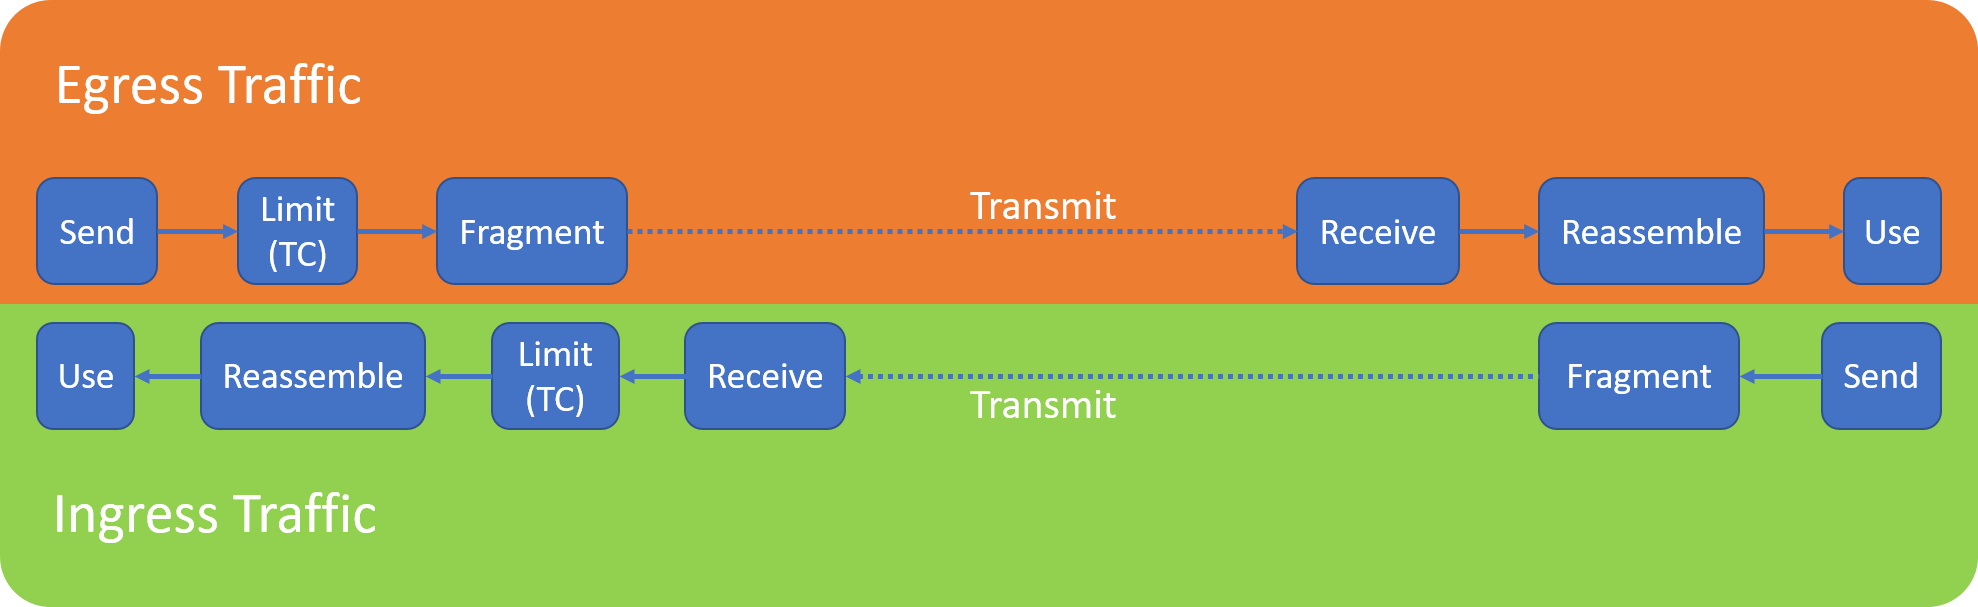
\includegraphics[width=\textwidth]{img/Fragmentation.png}
	\caption{Schematic Representation of where Fragmentation occurs}
	\label{Schematic Representation of where Fragmentation occurs}
\end{figure}

To figure out whether the previously mentioned hypothesis holds, we again run two different tests.
\\
This time we fix the datagram size and vary the target bandwidth from 100 Kbps to 1000 Kbps (option \textit{-b}). The upper limit for the bandwidth is still 500 Kbps and has been enforced using the \textit{scionlab\_bw\_limiter}. 
\\
For the first test, we set a datagram size of 10000 bytes, while having a \acs{MTU} of 1500 bytes. Therefore, fragmentation is going to happen in this case. Figure \ref{Evaluation of the Bandwidth with a Datagram Size of 10000 Bytes} shows the results of this test. It is visible that as long as the target bandwidth is below the bandwidth limit of 500 Kbps, ingress traffic reaches the desired target bandwidth. However, as soon as we try to send traffic at a higher rate than the enforced limit, we see the significant drop in bandwidth that we observed beforehand. As figure \ref{Evaluation of Bandwidth Drops with a Datagram Size of 100000 Bytes} shows, a lot of samples experience a bandwidth drop to a bandwidth of zero as soon as they try to reach a bandwidth above the enforced limit. For egress traffic, iPerf3 fails to reach such a low target bandwidth, because it tries to send at least 10 datagrams per second, with each datagram having the specified size. Therefore, the effective bandwidth for egress traffic is: 
$$\text{effective bandwidth} = max\left\lbrace\frac{10\cdot \text{datagram size}}{1}\left[ \frac{bytes}{second} \right],\text{target bandwidth}\right\rbrace$$ 

The fact that ingress traffic behaves as expected if we have a target bandwidth which is below the enforced limit, regardless of the datagram size, shows that the enforced limit is responsible for the bandwidth drop of ingress traffic. To make sure that this drop is caused by fragmentation and not by wrong \acs{TC} configurations, we run a second test, where we set the datagram size to the size of the \acs{MTU}. If the hypothesis is valid and the bandwidth drop is caused by fragmentation, then we should see that the reached bandwidth is what we expect, namely the minimum of the bandwidth limit and the target bandwidth.

\begin{figure}[h]
	\centering
	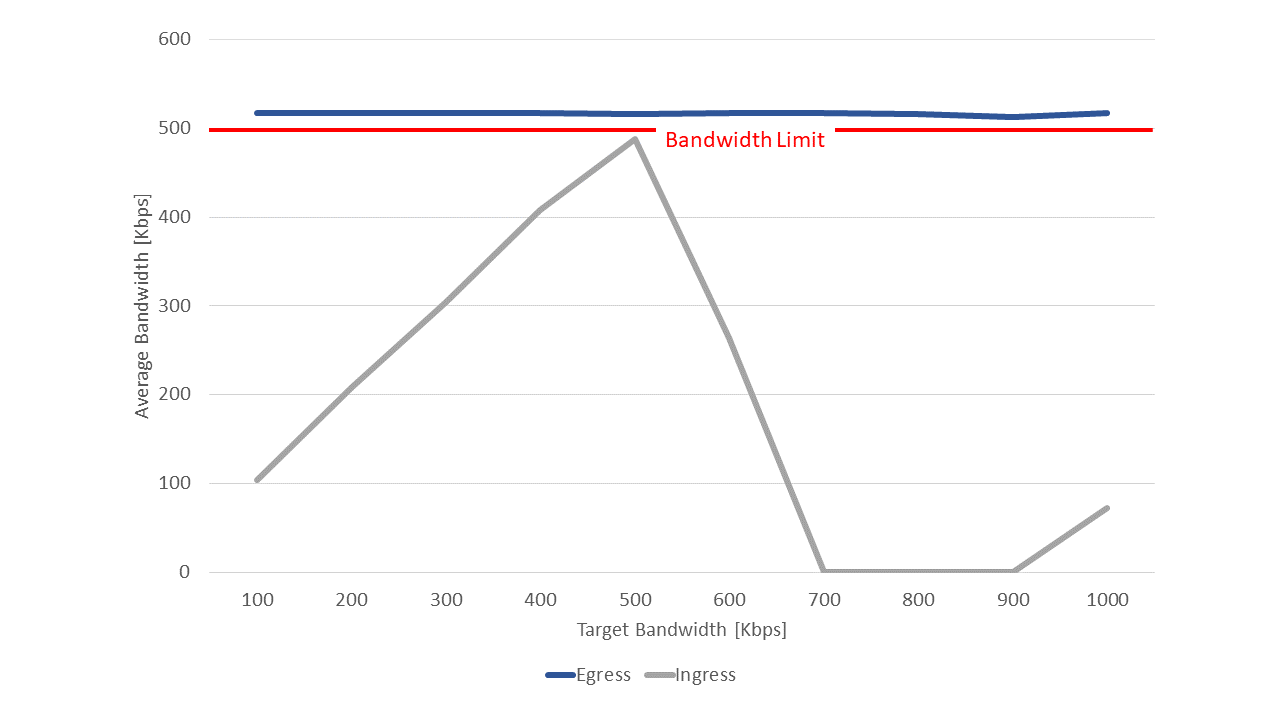
\includegraphics[width=\textwidth]{img/Evaluation-Bandwidth-Big-Buffer.png}
	\caption{Evaluation of the Bandwidth with a Datagram Size of 10000 Bytes}
	\label{Evaluation of the Bandwidth with a Datagram Size of 10000 Bytes}
\end{figure}

\begin{figure}[h]
	\centering
	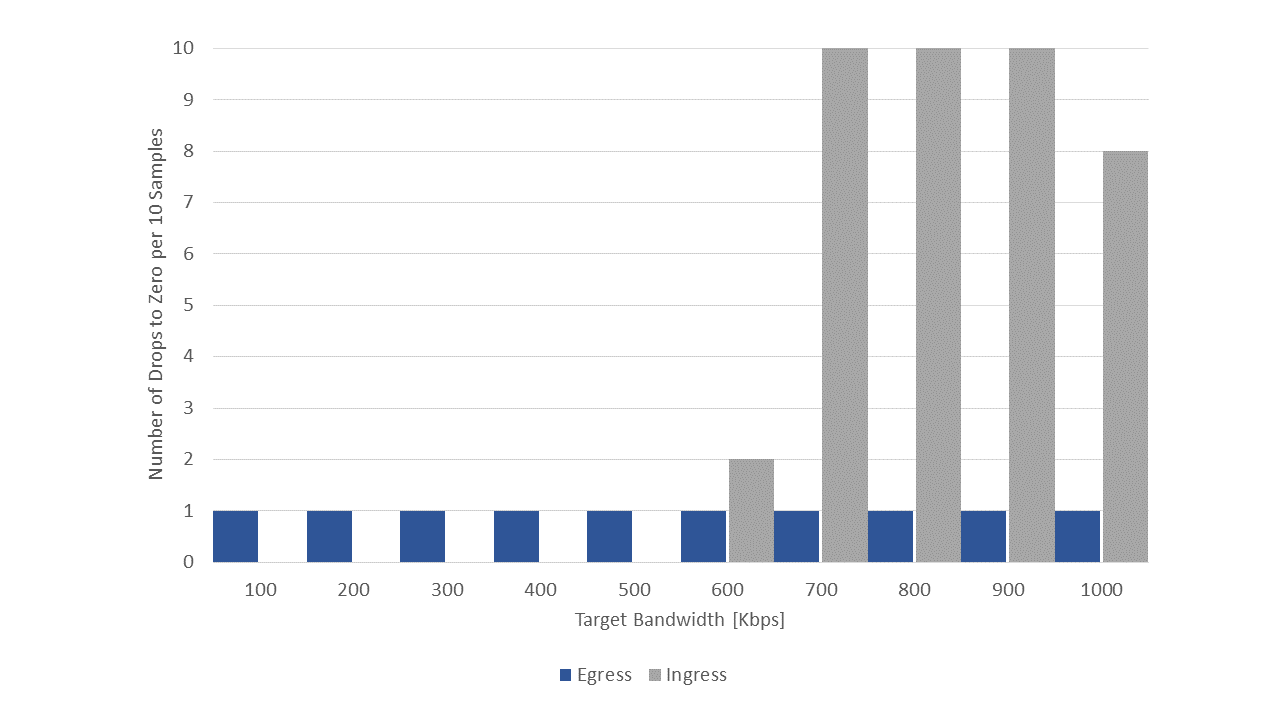
\includegraphics[width=\textwidth]{img/Evaluation-Zeros-Big-Buffer.png}
	\caption{Evaluation of Bandwidth Drops with a Datagram Size of 100000 Bytes}
	\label{Evaluation of Bandwidth Drops with a Datagram Size of 100000 Bytes}
\end{figure}
\newpage

For the second test, we set the datagram size to 1500 bytes, which is the size of the \acs{MTU}. As visible in figure \ref{Evaluation of the Bandwidth with a Datagram Size of 1500 Bytes (Size of the MTU)}, both ingress as well as egress traffic first reach the target bandwidth, for as long as it is below the enforced bandwidth limit, and then it stabilizes approximately around the bandwidth limit. As expected, egress traffic stabilizes slightly above the enforced limit, because we allow short bursts at a higher bandwidth. Ingress traffic stabilizes as well, but also as expected slightly below the enforced bandwidth limit, because there is a certain overhead caused by redirecting ingress traffic to a virtual interface.
\\
Therefore, we can conclude that the previously discovered strange behaviour of ingress traffic is not a side effect of the \textit{scionlab\_bw\_limiter} but instead is normal behaviour that is caused by fragmentation (see section \ref{Fragmentation shown using Wireshark} for further clarification). Since our goal was to limit the bandwidth the same way a slow link would, we have to accept this behaviour and can therefore say that the bandwidth limitation was enforced successfully.

\begin{figure}[h]
	\centering
	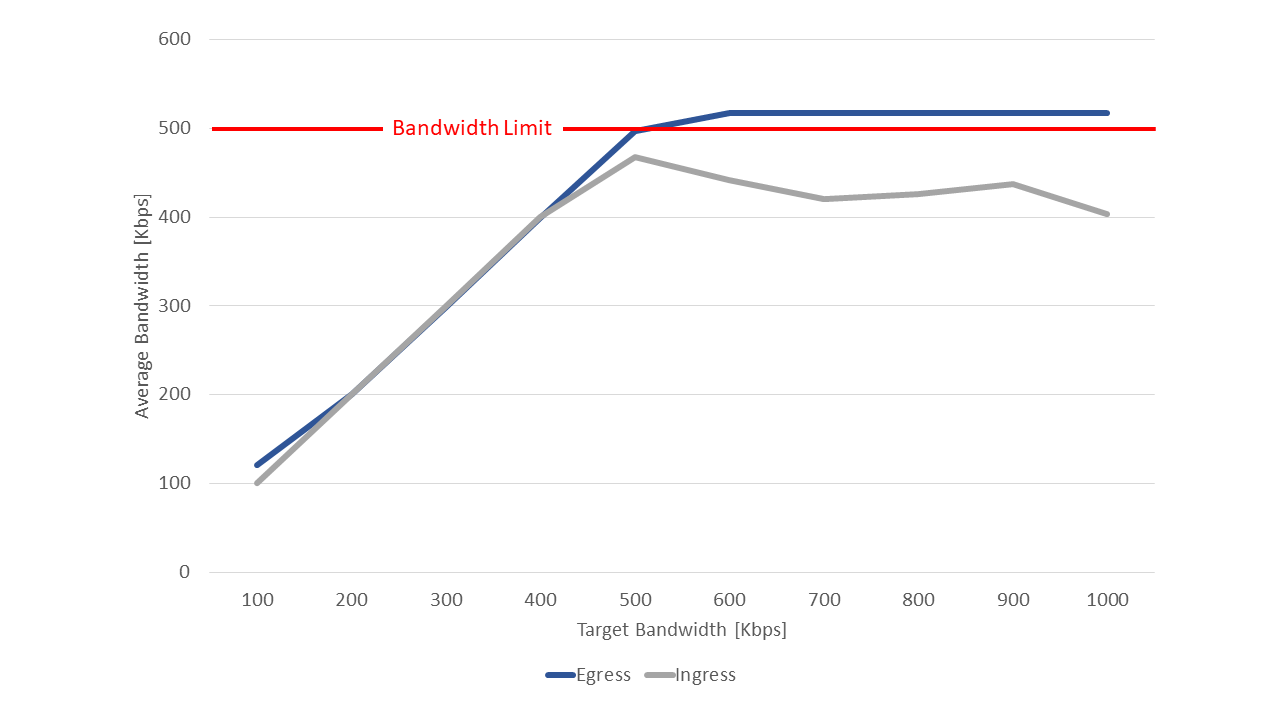
\includegraphics[width=\textwidth]{img/Evaluation-Bandwidth-Small-Buffer.png}
	\caption{Evaluation of the Bandwidth with a Datagram Size of 1500 Bytes (Size of the MTU)}
	\label{Evaluation of the Bandwidth with a Datagram Size of 1500 Bytes (Size of the MTU)}
\end{figure}

\newpage

\subsection{Fragmentation shown using Wireshark}\label{Fragmentation shown using Wireshark}

Wireshark is a state of the art network traffic analyser. It is open source and its source code can be found on \href{https://github.com/wireshark/wireshark}{github.com}\cite{combs2019wireshark}. We use wireshark to visualize ingress traffic that has been generated by iPerf3 and goes from our test server to the test client. Listing \ref{Example, where no Fragmentation occurs} and \ref{Example, where Fragmentation occurs} show the iPerf3 commands used to generate the traffic, which is visualized in figure \ref{Wireshark Output, where no Fragmentation occurs} and \ref{Wireshark Output, where Fragmentation occurs} respectively.
\\
In the first test (listing \ref{Example, where no Fragmentation occurs}), we set the datagram size to 1000 bytes, which is smaller than the size of the \acs{MTU} (which is 1500 bytes). In this case, we observe that no fragmentation of the test traffic occurs. Therefore, as visible in figure \ref{Wireshark Output, where no Fragmentation occurs}, each arriving \acs{IP}-frame results in a valid \acs{UDP}-datagram.
\\
However, if we set the datagram size to 10000 bytes (listing \ref{Example, where Fragmentation occurs}), then a \acs{UDP}-datagram needs to be fragmented into $\left\lceil\frac{10000}{1500}\right\rceil = 7$ \acs{IP}-frames. As visible in figure \ref{Wireshark Output, where Fragmentation occurs}, the first couple of frames get successfully reassembled into a valid datagram, where as at some point, here at packet number 48, the limitations start taking effect and no longer every \acs{IP}-frame gets received. As visible in the right most column of figure \ref{Wireshark Output, where Fragmentation occurs}, \acs{UDP}-datagrams can no longer be successfully reassembled, which leads to many incomplete and therefore invalid datagrams.

\newpage

\begin{lstlisting}[language=sh, caption = {Example, where no Fragmentation occurs}, captionpos=b, numbers=left, frame=single, breaklines=true, breakatwhitespace=true, showstringspaces=false, label={Example, where no Fragmentation occurs}]
iperf3 -c 192.168.17.129 -u -b 2Mbit -l 1000 -R
\end{lstlisting}

\begin{figure}[h]
	\centering
	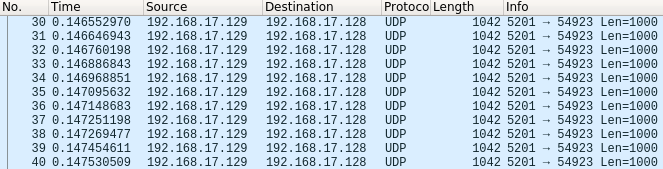
\includegraphics[width=\textwidth]{img/wireshark_l_1000_b_2Mbit.png}
	\caption{Wireshark Output, where no Fragmentation occurs}
	\label{Wireshark Output, where no Fragmentation occurs}
\end{figure}

\begin{lstlisting}[language=sh, caption = {Example, where Fragmentation occurs}, captionpos=b, numbers=left, frame=single, breaklines=true, breakatwhitespace=true, showstringspaces=false, label={Example, where Fragmentation occurs}]
iperf3 -c 192.168.17.129 -u -b 1Gbit -l 10000 -R
\end{lstlisting}

\begin{figure}[h]
	\centering
	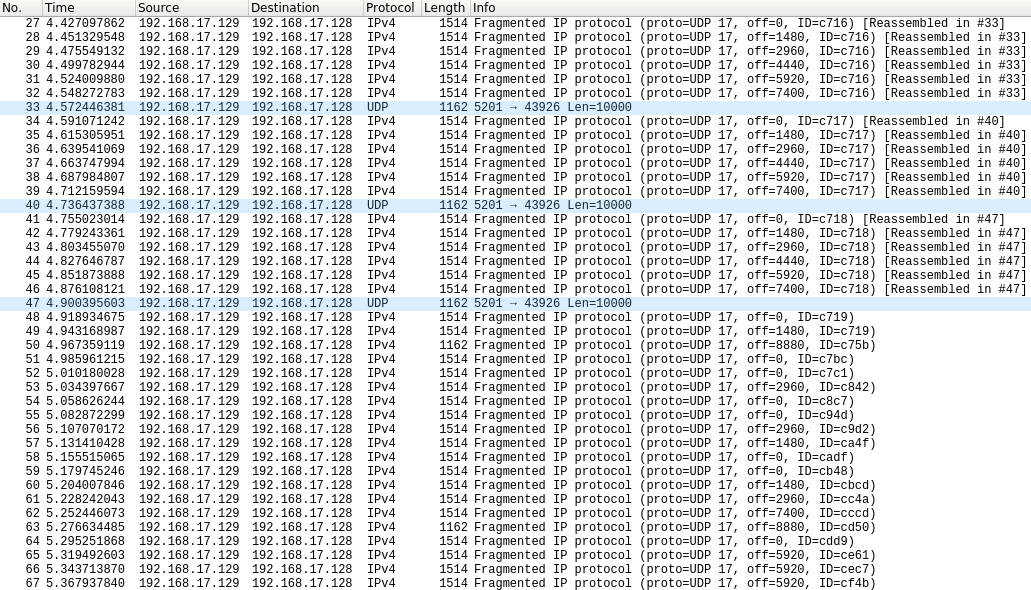
\includegraphics[width=\textwidth]{img/wireshark_l_10000_b_1Gbit.png}
	\caption{Wireshark Output, where Fragmentation occurs}
	\label{Wireshark Output, where Fragmentation occurs}
\end{figure}